\documentclass[a4paper,9pt]{extarticle}

%=========================================================
% PACKAGES
%=========================================================

\usepackage[
a4paper,
top=1.8cm,
bottom=1.5cm,
footskip=7mm,
left=1cm,
right=1cm,
headheight=14pt,
headsep=5mm
]{geometry}

\usepackage[T1]{fontenc}
\usepackage[utf8]{inputenc}
\usepackage[french]{babel}

\usepackage[sfdefault]{FiraSans}
\renewcommand{\familydefault}{\sfdefault}

\usepackage{multicol}
\setlength{\columnsep}{0.7cm}

\usepackage{amsmath,amssymb}
\usepackage{titlesec}
\usepackage{enumitem}

\usepackage{tcolorbox}
\tcbuselibrary{skins,breakable}

\usepackage{xcolor}
\usepackage{graphicx}
\usepackage{float}
\usepackage{tikz}

\usepackage{fancyhdr}
\usepackage[hidelinks]{hyperref}


%=========================================================
% PAGE SETTINGS
%=========================================================

\setlength{\parindent}{0pt}
\setlength{\parskip}{1.5pt}

\setlength{\abovedisplayskip}{4pt}
\setlength{\belowdisplayskip}{4pt}

\setlist[itemize]{
leftmargin=*,
itemsep=1pt,
topsep=1pt
}


%=========================================================
% COLORS
%=========================================================

\definecolor{Blue}{HTML}{E3F0FF}
\definecolor{Green}{HTML}{E3F7EA}
\definecolor{Pink}{HTML}{FFE5ED}
\definecolor{Orange}{HTML}{FFF0DC}
\definecolor{Purple}{HTML}{EEE7FF}
\definecolor{Yellow}{HTML}{FFFADB}

\definecolor{BlueTitle}{HTML}{285B8F}
\definecolor{GreenTitle}{HTML}{287052}
\definecolor{PinkTitle}{HTML}{A84063}
\definecolor{OrangeTitle}{HTML}{A96500}
\definecolor{PurpleTitle}{HTML}{6245A5}


%=========================================================
% HEADER
%=========================================================

\pagestyle{fancy}
\fancyhf{}

\fancyhead[L]{\small\textbf{Electronique I}}
\fancyhead[C]{\small Impédances et nombres complexes}
\fancyhead[R]{\small Week 05 -- 05-11/10/2026}

\fancyfoot[C]{\small\href{https://github.com/AlphaXT38G/notes_ba5}{github.com/AlphaXT38G/notes\_ba5}}
\fancyfoot[R]{\small \thepage}

\renewcommand{\headrulewidth}{0.4pt}


%=========================================================
% TITLES
%=========================================================

\titleformat{\section}
{\large\bfseries\color{BlueTitle}}
{}{0pt}{}

\titlespacing{\section}
{0pt}{6pt}{3pt}


%=========================================================
% SEPARATOR
%=========================================================

\newcommand{\separator}{
\vspace{2pt}
\hrule
\vspace{3pt}
}


%=========================================================
% BOXES
%=========================================================

% DEFINITION - blue

\newtcolorbox{definition}{
enhanced,
breakable,
colback=Blue,
colframe=BlueTitle,
boxrule=0.7pt,
arc=0mm,
title=\textbf{Definition},
fonttitle=\bfseries
}


% IMPORTANT - pink

\newtcolorbox{important}{
enhanced,
breakable,
colback=Pink,
colframe=PinkTitle,
boxrule=0.7pt,
arc=0mm,
title=\textbf{Key idea},
fonttitle=\bfseries
}


% FORMULAS - green

\newtcolorbox{formula}{
enhanced,
breakable,
colback=Green,
colframe=GreenTitle,
boxrule=0.7pt,
arc=0mm,
title=\textbf{Key formulas},
fonttitle=\bfseries
}


% WARNING - orange

\newtcolorbox{warning}{
enhanced,
breakable,
colback=Orange,
colframe=OrangeTitle,
boxrule=0.7pt,
arc=0mm,
title=\textbf{Warning},
fonttitle=\bfseries
}


% EXAMPLE - purple

\newtcolorbox{example}{
enhanced,
breakable,
colback=Purple,
colframe=PurpleTitle,
boxrule=0.7pt,
arc=0mm,
title=\textbf{Example},
fonttitle=\bfseries
}


% SUMMARY - yellow

\newtcolorbox{summary}{
enhanced,
breakable,
colback=Yellow,
colframe=OrangeTitle,
boxrule=0.7pt,
arc=0mm,
title=\textbf{Summary},
fonttitle=\bfseries
}


% a box only breaks once it has a few lines on this column: no lone title at the bottom
\tcbset{lines before break=8}


%=========================================================
% DOCUMENT
%=========================================================

\begin{document}

\thispagestyle{fancy}

\footnotesize

\begin{multicols}{2}


%=========================================================
\section{Introduction : où on en est}


\begin{center}

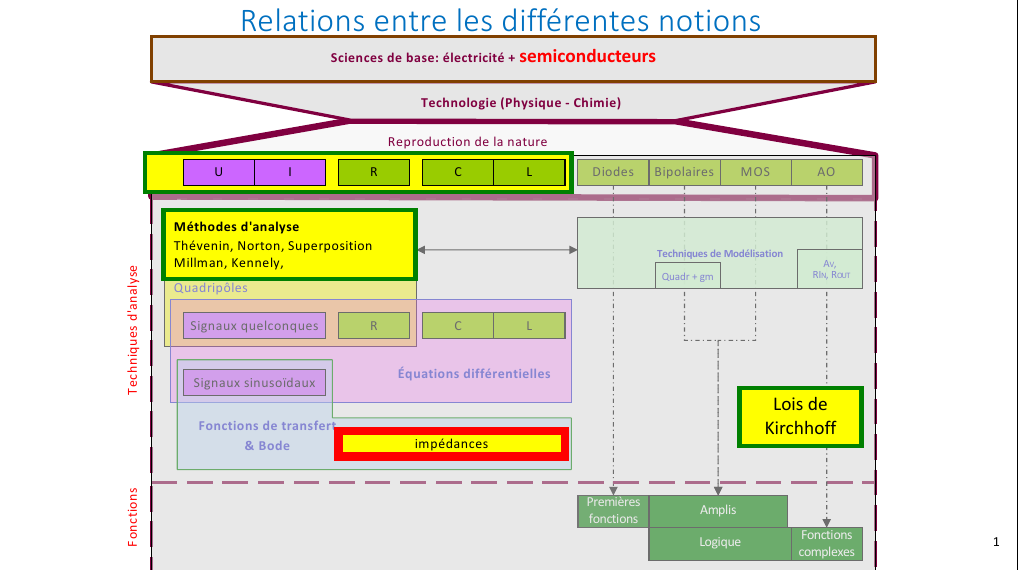
\includegraphics[
width=1.0\linewidth
]{../images/week05_01.png}

\end{center}

Le cours sur la modélisation de dipôles et quadripôles est un passage délicat car abstrait à ce stade de la formation. On revient à une approche plus classique exploitant l'outil mathématique.

Le cours va permettre de prédire le comportement de circuits composés de résistances et de condensateurs. Les deux types de signaux les plus utilisés pour caractériser ces circuits sont les signaux \textbf{sinusoïdaux} et \textbf{carrés}, utilisés respectivement en analogique et en numérique. Ce cours exploite les \textbf{expressions complexes} pour décrire le comportement de ces circuits. Cette notation évite deux difficultés majeures :

\begin{itemize}

\item décrire le comportement du circuit à partir d'équations différentielles ;

\item manipuler des expressions véhiculant, lorsqu'il s'agit de sinus, à la fois des amplitudes et des phases, ce qui s'avère complexe lors de la comparaison entre deux signaux (entrée et sortie).

\end{itemize}


\begin{center}

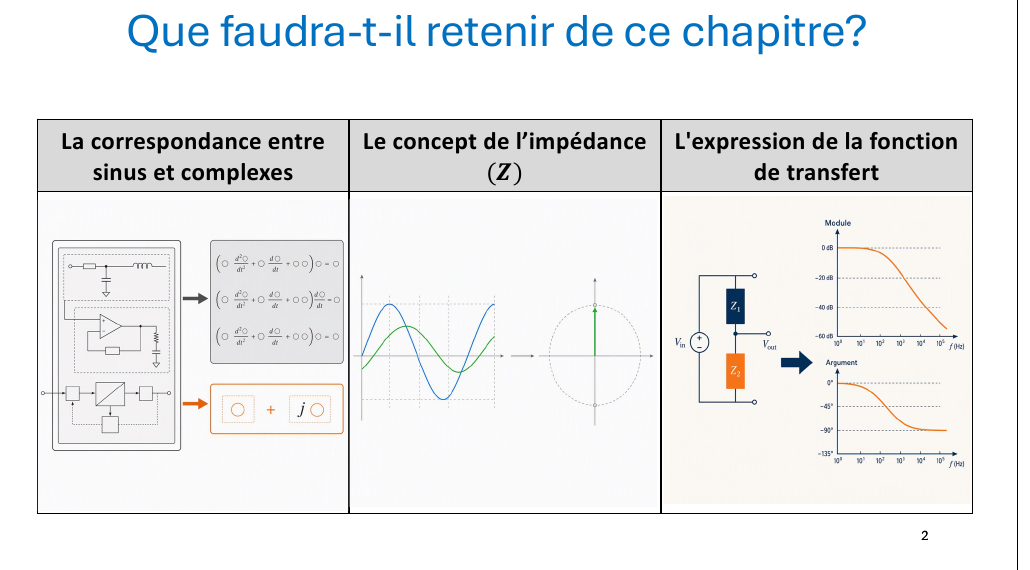
\includegraphics[
width=1.0\linewidth
]{../images/week05_02.png}

\end{center}


\begin{summary}

\textbf{Que faudra-t-il retenir de ce chapitre ?}

\begin{enumerate}[leftmargin=*,itemsep=1pt,topsep=1pt]

\item \textbf{La correspondance entre sinus et complexes :} un réseau de résistances soumis à un signal sinusoïdal reste régi par une loi d'Ohm sans la moindre difficulté. Mais dès qu'on y ajoute des capacités et/ou des inductances, la mise en équation fait apparaître des équations différentielles temporelles bien plus difficiles à résoudre. Heureusement, le régime sinusoïdal permet d'utiliser un outil mathématique très efficace : le \textbf{plan complexe}.

\item \textbf{Le concept de l'impédance ($Z$) :} étudiés séparément avec un sinus, le condensateur et l'inductance provoquent un déphasage strict entre le courant et la tension. En notation complexe, leur comportement s'assimile à une résistance imaginaire, dont la valeur varie avec la fréquence : c'est l'\textbf{impédance complexe}.

\item \textbf{L'expression de la fonction de transfert :} en associant ces impédances, on recrée des structures familières comme les diviseurs de tension. Le résultat n'est plus un simple rapport constant, mais une \textbf{fonction de transfert} : elle montre, selon la fréquence, l'atténuation exacte du signal et le déphasage produit entre l'entrée et la sortie.

\end{enumerate}

\end{summary}


\begin{important}

\textbf{En très simple : de quoi parle ce chapitre ?}

Jusqu'ici, avec des résistances, tout était facile : $U = R\,I$, une simple multiplication. Mais dès qu'on met un condensateur ou une bobine, les formules deviennent des \textbf{dérivées} et des \textbf{intégrales} (semaine 03), et c'est pénible à calculer.

\vspace{3pt}

Bonne nouvelle : quand le signal est un sinus (une vague régulière), il existe une astuce. On écrit les tensions et les courants avec des \textbf{nombres complexes}, et alors le condensateur et la bobine se comportent comme des \og résistances spéciales \fg{} (les \textbf{impédances}). On retrouve des calculs aussi simples que $U = Z\,I$, et on peut réutiliser tout ce qu'on sait : séries, parallèles, diviseurs, Millman, Thévenin\dots

\vspace{3pt}

Le chapitre se fait en 3 étapes : (1) voir pourquoi le condensateur et la bobine \og décalent \fg{} le sinus, (2) apprendre les nombres complexes qui gèrent ce décalage, (3) s'en servir pour calculer des circuits (filtres).

\end{important}


%=========================================================
\section{Rappels composants R, C, L}


\begin{center}

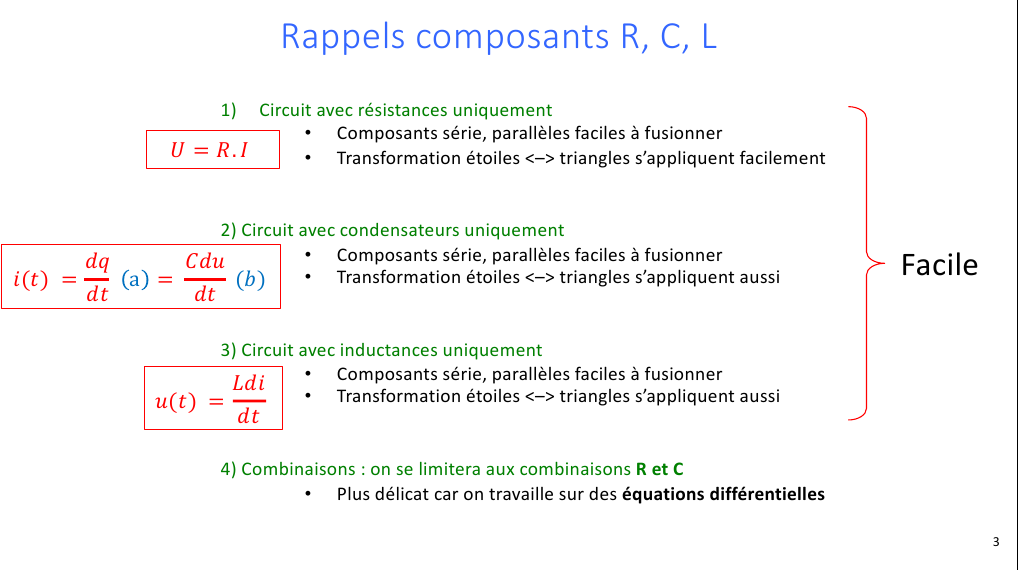
\includegraphics[
width=1.0\linewidth
]{../images/week05_03.png}

\end{center}


\begin{formula}

\[
U = R\,I
\qquad
i(t) = \frac{dq}{dt} = C\,\frac{du}{dt}
\qquad
u(t) = L\,\frac{di}{dt}
\]

où :

\begin{itemize}

\item $U$, $u(t)$ : tension [V] ; $I$, $i(t)$ : courant [A] ;

\item $R$ : résistance [$\Omega$] ; $C$ : capacité [F] ; $L$ : inductance [H] ;

\item $q$ : charge [C] ; $t$ : temps [s].

\end{itemize}

\end{formula}


Le degré de complexité n'est pas le même selon que l'on analyse :

\begin{itemize}

\item \textbf{des résistances uniquement} : les équations sont linéaires et basées sur la loi d'Ohm ; séries et parallèles faciles à fusionner, transformations étoile $\leftrightarrow$ triangle faciles ;

\item \textbf{des condensateurs uniquement} : en exploitant la notion de charge ($Q = CV$), on décrit aussi un système linéaire (même facilité) ;

\item \textbf{des inductances uniquement} : même facilité ;

\item \textbf{une combinaison de résistances et de condensateurs} : plus délicat, car elle met en évidence des \textbf{équations différentielles} (du premier ordre pour un seul condensateur).

\end{itemize}

La combinaison RL donne la même complexité, et RLC des équations du second ordre. Dans ce cours, on se limite aux combinaisons \textbf{R et C}.


\begin{important}

\textbf{En très simple}

Un seul type de composant à la fois, c'est facile : que des résistances, que des condensateurs ou que des bobines, on fusionne tout comme d'habitude.

\vspace{3pt}

Le problème arrive quand on \textbf{mélange} : la résistance obéit à une simple multiplication ($U = RI$), mais le condensateur obéit à une dérivée ($i = C\,du/dt$). Mettre les deux dans la même équation donne une équation où apparaissent une grandeur et sa dérivée : une équation différentielle, difficile à résoudre à la main. Tout le chapitre sert à éviter ça.

\end{important}


\end{multicols}

\end{document}
